\documentclass[12pt,a4paper]{article}
\usepackage[utf8]{vietnam}
\usepackage{amsmath,amssymb}
\usepackage{tabularx}
\usepackage{graphicx}
\usepackage{tikz}
\usetikzlibrary{calc,arrows.meta}
\usepackage{xcolor}
\usepackage{enumitem}
\usepackage{fancyhdr}
\usepackage[top=0.8cm, bottom=0.8cm, left=1.2cm, right=1.2cm]{geometry}
\usepackage[dethi]{ex_test}
\SAOPTN{widthSA=2.6,heightSA=0.62}

\setlength{\headheight}{15pt}
\setlength{\parskip}{0pt}

\pagestyle{fancy}
\fancyhf{}
\rhead{\textit{Môn Toán 7 -- Đề số 14}}
\lhead{\textit{Bộ đề ôn tập Giữa học kì I}}
\cfoot{\thepage}

\begin{document}

% --- KHUNG TIÊU ĐỀ ĐỀ THI ---
\noindent
\begin{tabularx}{\linewidth}{X r}
\textbf{TRƯỜNG THCS: \dotfill} & \textbf{ĐỀ KIỂM TRA ĐỊNH KỲ GIỮA HỌC KỲ I} \\
\textbf{Họ và tên: \dotfill} & \textbf{NĂM HỌC 2026 -- 2027} \\
\textbf{Lớp: \dotfill \quad SBD: \dotfill} & \textbf{Môn: TOÁN 7} \\
& \textit{Thời gian làm bài: 90 phút (không kể thời gian phát đề)}
\end{tabularx}

\vspace{1mm}
\noindent
\begin{tabularx}{\linewidth}{|p{3.5cm}|X|}
\hline
\centering\textbf{Điểm số} & \centering\textbf{Lời nhận xét của thầy cô giáo} \tabularnewline
\rule{0pt}{0.8cm} & \\
\hline
\end{tabularx}

\vspace{1.5mm}
\begin{center}
\textbf{\large ĐỀ SỐ 14}
\end{center}

\noindent\textbf{\large PHẦN I. CÂU TRẮC NGHIỆM NHIỀU PHƯƠNG ÁN LỰA CHỌN (3,0 điểm)}

\textit{Thí sinh trả lời từ câu 1 đến câu 12. Mỗi câu hỏi chỉ chọn một phương án đúng nhất và ghi vào bảng đáp án.}

\vspace{1mm}
\begin{ex}
Phát biểu nào sau đây là đúng?
\choice
{$\sqrt{2} \in \mathbb{Q}$}
{$-5 \notin \mathbb{Q}$}
{$-\dfrac{5}{4} \notin \mathbb{Q}$}
{\True $\dfrac{3}{2} \in \mathbb{Q}$}
\end{ex}

\begin{ex}
Số giá trị nguyên của $x$ thỏa mãn $-\dfrac{2}{3} < \dfrac{x}{12} < -\dfrac{1}{4}$ là:
\choice
{$3$}
{$2$}
{$5$}
{\True $4$}
\end{ex}

\begin{ex}
Số $9$ có căn bậc hai số học là:
\choice
{$3$ và $-3$}
{\True $3$}
{$-3$}
{$18$}
\end{ex}

\begin{ex}
\immini{
Cho hình vẽ bên, biết $OB$ là tia phân giác của $\widehat{AOC}$. Khi đó số đo của $\widehat{AOB}$ là:
\choice
{$65^\circ$}
{\True $32^\circ$}
{$130^\circ$}
{$18^\circ$}
}{
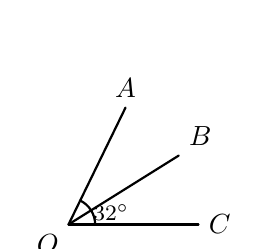
\begin{tikzpicture}[scale=0.75, line cap=round, line join=round]
    \coordinate (O) at (0,0);
    \coordinate (C) at (2.2,0);
    \coordinate (B) at (32:2.2);
    \coordinate (A) at (64:2.2);
    \draw[thick] (O) -- (C) node[right] {$C$};
    \draw[thick] (O) -- (B) node[above right] {$B$};
    \draw[thick] (O) -- (A) node[above] {$A$};
    \node[below left] at (O) {$O$};
    \draw[thick] (O) ++(0:0.45) arc (0:32:0.45);
    \node[font=\footnotesize] at (16:0.75) {$32^\circ$};
    \draw[thick] (O) ++(32:0.45) arc (32:64:0.45);
\end{tikzpicture}
}
\end{ex}

\begin{ex}
Kết quả của phép tính $\left(-\dfrac{1}{3}\right)^{2024} : \left(-\dfrac{1}{3}\right)^{2022}$ là:
\choice
{$\dfrac{1}{3}$}
{$-\dfrac{1}{9}$}
{\True $\dfrac{1}{9}$}
{$-\dfrac{2}{3}$}
\end{ex}

\begin{ex}
\immini{
Quan sát trục số bên dưới và chọn đáp án đúng về giá trị của điểm $a$:
\choice
{$a = \dfrac{1}{3}$}
{$a = \dfrac{1}{2}$}
{$a = \dfrac{2}{5}$}
{\True $a = \dfrac{2}{3}$}
}{
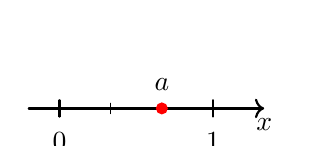
\begin{tikzpicture}[scale=1.3, line cap=round, line join=round]
    \draw[thick, ->] (-0.3,0) -- (2.0,0) node[below] {$x$};
    \draw[thick] (0, 0.08) -- (0, -0.08) node[below=2pt] {$0$};
    \draw[thick] (1.5, 0.08) -- (1.5, -0.08) node[below=2pt] {$1$};
    \draw (0.5, 0.05) -- (0.5, -0.05);
    \draw (1.0, 0.05) -- (1.0, -0.05);
    \filldraw[red] (1.0, 0) circle (1.5pt) node[above=3pt, black] {$a$};
\end{tikzpicture}
}
\end{ex}

\begin{ex}
Trong các số $\dfrac{9}{7}; 0{,}2; 0; -\dfrac{13}{5}; \dfrac{3}{15}; -\dfrac{2}{5}; -\dfrac{8}{5}$, có bao nhiêu số hữu tỉ dương?
\choice
{$1$}
{\True $3$}
{$2$}
{$4$}
\end{ex}

\begin{ex}
Cho $\widehat{xOy} = 80^\circ$. Góc đối đỉnh với $\widehat{xOy}$ có số đo độ là:
\choice
{$50^\circ$}
{\True $80^\circ$}
{$100^\circ$}
{$120^\circ$}
\end{ex}

\newpage
\begin{ex}
Các mặt của hình lập phương đều là:
\choice
{\True Hình vuông}
{Tam giác đều}
{Hình chữ nhật}
{Hình thoi}
\end{ex}

\begin{ex}
\immini{
Cho hình vẽ bên, biết $\widehat{CFE} = 60^\circ, \widehat{E}_1 = 120^\circ$. Xét hai khẳng định: (I) $\widehat{BEF} = 60^\circ$; (II) $AB \parallel CD$. Khẳng định nào sau đây là đúng?
\choice
{Chỉ (I) đúng}
{Chỉ (II) đúng}
{\True Cả (I) và (II) đều đúng}
{Cả (I) và (II) đều sai}
}{
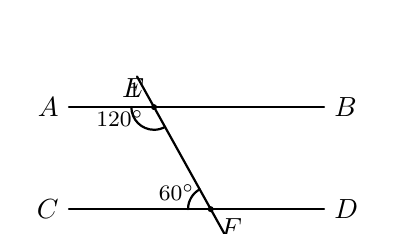
\begin{tikzpicture}[scale=0.72, line cap=round, line join=round]
    \draw[thick] (-2, 1.8) node[left] {$A$} -- (2.5, 1.8) node[right] {$B$};
    \draw[thick] (-2, 0) node[left] {$C$} -- (2.5, 0) node[right] {$D$};
    \coordinate (E) at (-0.5, 1.8);
    \coordinate (F) at (0.5, 0);
    \draw[thick] ($(E)!-0.3!(F)$) -- ($(F)!-0.3!(E)$);
    \filldraw[black] (E) circle (1.2pt) node[above left] {$E$};
    \filldraw[black] (F) circle (1.2pt) node[below right] {$F$};
    % E1 = 120 (angle AEF)
    \draw[thick] (E) ++(180:0.4) arc (180:299.1:0.4);
    \node[font=\footnotesize] at ($(E)+(-0.6,-0.2)$) {$120^\circ$};
    \node[font=\footnotesize] at ($(E)+(-0.35,0.3)$) {$1$};
    % CFE = 60
    \draw[thick] (F) ++(180:0.4) arc (180:119.1:0.4);
    \node[font=\footnotesize] at ($(F)+(-0.6,0.3)$) {$60^\circ$};
\end{tikzpicture}
}
\end{ex}

\begin{ex}
Hai đường thẳng $xx'$ và $yy'$ cắt nhau tại $O$. Góc đối đỉnh với $\widehat{x'Oy}$ là:
\choice
{\True $\widehat{xOy'}$}
{$\widehat{x'Oy}$}
{$\widehat{x'Oy'}$}
{$\widehat{xOy}$}
\end{ex}

\begin{ex}
Cho ba đường thẳng phân biệt $a, b, c$ biết $a \parallel c$ và $b \parallel c$. Kết luận nào sau đây là đúng?
\choice
{$a$ cắt $b$}
{\True $a \parallel b$}
{$a \perp b$}
{$a$ trùng $b$}
\end{ex}


\vspace{1mm}
\noindent\textbf{BẢNG TRẢ LỜI TRẮC NGHIỆM PHẦN I:}
\begin{center}
\begin{tabular}{|c|c|c|c|c|c|c|c|c|c|c|c|c|}
\hline
\textbf{Câu} & \textbf{1} & \textbf{2} & \textbf{3} & \textbf{4} & \textbf{5} & \textbf{6} & \textbf{7} & \textbf{8} & \textbf{9} & \textbf{10} & \textbf{11} & \textbf{12} \\
\hline
\textbf{Chọn} & \rule{0pt}{0.48cm} & & & & & & & & & & & \\
\hline
\end{tabular}
\end{center}
\vspace{1mm}

\setcounter{ex}{0}
\noindent\textbf{\large PHẦN II. CÂU TRẮC NGHIỆM ĐÚNG SAI (2,0 điểm)}

\textit{Thí sinh trả lời câu 1 và câu 2. Trong mỗi ý a), b), c), d) ở mỗi câu, thí sinh chọn đúng hoặc sai.}

\vspace{1mm}
\begin{ex}
Cho biểu thức $P = \dfrac{3}{5} \cdot \left(-\dfrac{5}{6}\right) + \left(-\dfrac{1}{2}\right)^2 - \left|-\dfrac{3}{4}\right|$. Xét tính đúng sai của các mệnh đề sau:
\choiceTF
{\True Giá trị của phép nhân $\dfrac{3}{5} \cdot \left(-\dfrac{5}{6}\right)$ bằng $-\dfrac{1}{2}$}
{Giá trị của lũy thừa $\left(-\dfrac{1}{2}\right)^2$ bằng $-\dfrac{1}{4}$}
{\True Giá trị tuyệt đối $\left|-\dfrac{3}{4}\right|$ bằng $\dfrac{3}{4}$}
{\True Giá trị của biểu thức $P$ bằng $-1$}
\end{ex}

\begin{ex}
\immini{
Quan sát hình vẽ bên, biết đường thẳng $d \perp m$ tại $H$, $d \perp n$ tại $I$; đường thẳng $c$ cắt $m$ tại $A$ và cắt $n$ tại $B$ sao cho $\widehat{ABI} = 80^\circ$. Xét tính đúng sai của các mệnh đề sau:
\choiceTF
{\True Hai đường thẳng $m$ và $n$ song song với nhau ($m \parallel n$)}
{\True Góc so le trong với góc $\widehat{ABI}$ tại đỉnh $A$ có số đo bằng $80^\circ$}
{Góc trong cùng phía với góc $\widehat{ABI}$ tại đỉnh $A$ có số đo bằng $80^\circ$}
{\True Số đo góc $\widehat{AHI}$ bằng $90^\circ$}
}{
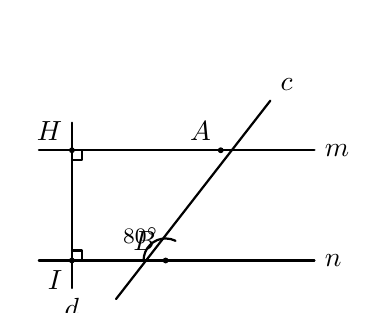
\begin{tikzpicture}[scale=0.7, line cap=round, line join=round]
    % Lines m and n
    \draw[thick] (-2.2, 2.0) -- (2.8, 2.0) node[right] {$m$};
    \draw[thick] (-2.2, 0) -- (2.8, 0) node[right] {$n$};
    % Line d perpendicular at H and I
    \draw[thick] (-1.6, 2.5) -- (-1.6, -0.5) node[below] {$d$};
    \filldraw[black] (-1.6, 2.0) circle (1.2pt) node[above left] {$H$};
    \filldraw[black] (-1.6, 0) circle (1.2pt) node[below left] {$I$};
    \draw[thick] (-1.6, 2.0) ++(0,-0.18) -- ++(0.18,0) -- ++(0,0.18);
    \draw[thick] (-1.6, 0) ++(0,0.18) -- ++(0.18,0) -- ++(0,-0.18);
    % Line c slanted cutting m at A, n at B
    \draw[thick] (2.0, 2.9) node[above right] {$c$} -- (-0.8, -0.7);
    \filldraw[black] (1.1, 2.0) circle (1.2pt) node[above left] {$A$};
    \filldraw[black] (0.1, 0) circle (1.2pt) node[above left] {$B$};
    % Angle ABI = 80
    \draw[thick] (0.1, 0) ++(180:0.4) arc (180:63.4:0.4);
    \node[font=\footnotesize] at (-0.35, 0.45) {$80^\circ$};
\end{tikzpicture}
}
\end{ex}


\noindent\textbf{BẢNG TRẢ LỜI PHẦN II:}
\begin{center}
\begin{tabular}{|c|c|c|c|c||c|c|c|c|c|}
\hline
\textbf{Câu 1} & \textbf{a)} & \textbf{b)} & \textbf{c)} & \textbf{d)} & \textbf{Câu 2} & \textbf{a)} & \textbf{b)} & \textbf{c)} & \textbf{d)} \\
\hline
\textbf{Đ/S} & \rule{0pt}{0.45cm} & & & & \textbf{Đ/S} & & & & \\
\hline
\end{tabular}
\end{center}
\vspace{1mm}

\setcounter{ex}{0}
\noindent\textbf{\large PHẦN III. CÂU HỎI TRẢ LỜI NGẮN (1,0 điểm)}

\textit{Thí sinh trả lời câu 1 và câu 2. Điền kết quả vào ô trống.}

\vspace{1mm}
\begin{ex}
Tìm số hữu tỉ $x$, biết: $3 \cdot \left(x - \dfrac{1}{4}\right) + \dfrac{1}{2} = \dfrac{1}{3}$. \shortans{$\dfrac{7}{36}$}
\end{ex}

\begin{ex}
\immini{
Cho hình hộp chữ nhật $ABCD.A'B'C'D'$ như hình vẽ có chiều dài $D'C' = 4\text{ cm}$, chiều rộng $B'C' = 2\text{ cm}$ và chiều cao $BB' = 3\text{ cm}$. Tính thể tích của hình hộp chữ nhật này.
\vspace{1mm}
\hfill\shortans{$24\text{ cm}^3$}
}{
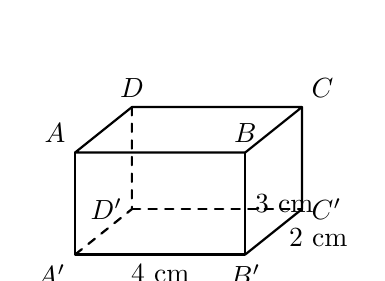
\begin{tikzpicture}[scale=0.72, line cap=round, line join=round]
    \coordinate (A) at (0, 1.8);
    \coordinate (B) at (3.0, 1.8);
    \coordinate (C) at (4.0, 2.6);
    \coordinate (D) at (1.0, 2.6);
    \coordinate (A_prime) at (0, 0);
    \coordinate (B_prime) at (3.0, 0);
    \coordinate (C_prime) at (4.0, 0.8);
    \coordinate (D_prime) at (1.0, 0.8);

    \draw[thick] (A) -- (B) -- (C) -- (D) -- cycle;
    \draw[thick] (A) -- (A_prime) -- (B_prime) -- (B);
    \draw[thick] (B_prime) -- (C_prime) -- (C);
    \draw[thick, dashed] (D) -- (D_prime) -- (A_prime);
    \draw[thick, dashed] (D_prime) -- (C_prime);

    \node[above left] at (A) {$A$};
    \node[above] at (B) {$B$};
    \node[above right] at (C) {$C$};
    \node[above] at (D) {$D$};
    \node[below left] at (A_prime) {$A'$};
    \node[below] at (B_prime) {$B'$};
    \node[right] at (C_prime) {$C'$};
    \node[left] at (D_prime) {$D'$};

    \node[below] at ($(A_prime)!0.5!(B_prime)$) {$4\text{ cm}$};
    \node[right] at ($(B_prime)!0.5!(C_prime)+(0.1,-0.1)$) {$2\text{ cm}$};
    \node[right] at ($(B)!0.5!(B_prime)$) {$3\text{ cm}$};
\end{tikzpicture}
}
\end{ex}


\newpage
\setcounter{ex}{0}
\noindent\textbf{\large PHẦN IV. TỰ LUẬN (4,0 điểm)}

\textit{Thí sinh trình bày chi tiết lời giải vào giấy làm bài.}

\vspace{1mm}
\begin{ex}
Tính giá trị các biểu thức sau (tính bằng cách hợp lý nếu có thể):
\begin{enumerate}[label=\textbf{\alph*)}, leftmargin=0.8cm, itemsep=1pt]
\item $A = \dfrac{2}{7} + \left(-\dfrac{3}{7}\right) : \dfrac{3}{2}$
\item $B = \dfrac{5}{17} \cdot \left(-\dfrac{31}{33}\right) + \dfrac{5}{17} \cdot \left(-\dfrac{2}{33}\right) + 2\dfrac{5}{17}$
\item $C = \sqrt{4} + \sqrt{9} + \sqrt{16} + \sqrt{25}$
\item $D = 0{,}(5) - 1\dfrac{1}{3} - 0{,}(7)$
\end{enumerate}
\end{ex}
\vspace{2mm}

\begin{ex}
Tìm $x$, biết:
\begin{enumerate}[label=\textbf{\alph*)}, leftmargin=0.8cm, itemsep=1pt]
\item $2x - \dfrac{1}{3} = \dfrac{5}{6}$
\item $\left(x - \dfrac{1}{2}\right)^2 = \dfrac{9}{25}$
\end{enumerate}
\end{ex}
\vspace{2mm}

\begin{ex}
Bể cá của quán cà phê Koi có dạng hình hộp chữ nhật có chiều dài $1{,}8\text{ m}$, chiều rộng $1{,}2\text{ m}$ và chiều cao $1{,}5\text{ m}$.
\begin{enumerate}[label=\textbf{\alph*)}, leftmargin=0.8cm, itemsep=1pt]
\item Tính diện tích xung quanh của bể cá.
\item Chủ quán đã đổ nước vào bể sao cho mực nước cách miệng bể $20\text{ cm}$. Hỏi chủ quán đã đổ vào bể bao nhiêu lít nước? (biết rằng ban đầu bể không có nước).
\end{enumerate}
\end{ex}
\vspace{2mm}

\begin{ex}
Cho hai biểu thức sau: $A = \dfrac{25^{800} \cdot 16^{60} \cdot 3^{2500}}{8^{80} \cdot 27^{60} \cdot 5^{1600}}$ và $B = 3^{2025}$. Hãy so sánh $A$ và $B$.
\end{ex}
\vspace{2mm}


\begin{center}
\rule{4cm}{0.4pt}\\
\textit{--- HẾT ---}
\end{center}
\end{document}
